\documentclass[10pt]{beamer}
\usetheme[progressbar=frametitle]{metropolis}
\usepackage{appendixnumberbeamer}
\usepackage{booktabs}
\usepackage[scale=2]{ccicons}
\usepackage{pgfplots}
\usepgfplotslibrary{dateplot}
\usepackage{xspace}
\usepackage{graphicx}
\usepackage[italian]{babel}
\usepackage{hyperref}
\usepackage{tikz}
\newcommand{\themename}{\textbf{\textsc{metropolis}}\xspace}

\title{Max-Flow}
\subtitle{Quantum adiabatic computing}
\date{A.A. 2022/2023}
\author{Nicola Barbaro (1070668) - Mario Bifulco (881727)}
\institute{Università degli studi di Torino - Ottimizzazione Combinatoria}
\titlegraphic{\hfill
\includegraphics[height=1.5cm]{img/nuovo_logo}}
\begin{document}

\maketitle

\setbeamertemplate{section in toc}[sections numbered]

\begin{frame}{Table of contents}
  \tableofcontents
\end{frame}

\section{Max-Flow}
\begin{frame}
  \frametitle{Problema di flusso massimo}

  Dato un grafo orientato $G = (V, E)$, anche chiamato \emph{rete di flusso}, 
  si richiede di trovare il valore massimo, del bene che si vuole schematizzare, 
  in grado di fluire nella rete dal nodo sorgente $s$ al nodo foce $t$. 

  Utilizzi tipici sono legati al trasporto di beni o l'instradamento su reti.

\end{frame}
\begin{frame}
  \frametitle{Formulazione matematica}

  \begin{equation*}
    \begin{array}{ll@{}ll}
      \text{massimizza}   & \displaystyle\sum_{(s, i) \in FS_{i}} x_{si} = x_{ts} & \;\;\;\;\;\;\;\;\; &(1)\\
      \text{soggetto a}   & \displaystyle\sum_{(h, i) \in BS_{i}} x_{hi} - \sum_{(i, h) \in FS_{i}} x_{ij} = 0 \;\;\;\;\;\;\;\;\; &    \forall i \in V \backslash \{s,t\}&(2)\\
                          & \left(\displaystyle\sum_{(i, t) \in BS_{t}} x_{it}\right) - x_{ts} = 0 & &(3)\\
                          &  x_{ts} - \displaystyle\sum_{(s,i) \in FS_{s}} x_{si} = 0 & &(4)\\
                          &0 \leq x_{ij} \leq u_{ij} & \forall (i,j) \in E &(5).
    \end{array}
  \end{equation*}

\end{frame}
\begin{frame}
  \frametitle{Vincoli del problema}

  \begin{enumerate}
    \item Si vuole massimizzare il flusso su un arco \emph{dummy}, senza capacità, che va dalla foce $t$ alla fonte $s$.
    \item Vincoli che permettono di rispettare la \emph{conservazione dei flussi}.
    \item Il flusso massimo trovato dal problema deve combaciare con la somma dei flussi entranti nella foce e con la somma dei flussi uscenti dalla fonte.
    \item Bisogna rispettare il \emph{vincolo di capacità}.
\end{enumerate}

\end{frame}
\subsection{Teorema Max-Flow Min-Cut}
\begin{frame}
  \frametitle{Problema del minimo taglio}

  Dato un grafo orientato $G = (V, E)$, si richiede di partizionare i vertici $V$ in modo che:

  \begin{enumerate}
    \item Il nodo sorgente e quello foce non appartengano alla stessa partizione.
    \item Considerando $N_s$, la partizione contenente la sorgente, e $N_t$, 
    la partizione del nodo foce, la somma degli archi con coda in $N_s$ e testa in $N_t$ deve essere minima.
  \end{enumerate}

\end{frame}
\begin{frame}
  \frametitle{Formulazione matematica}

  \begin{equation*}
      \begin{array}{ll@{}ll}
      \text{minimizza}    & \displaystyle\sum_{(i, j) \in E} \omega_{ij}u_{ij} &  &(1)\\
      \text{soggetto a}   & \displaystyle \pi_t - \pi_s \geq 1 &   &(2)\\
                          & \displaystyle \pi_i - \pi_j  + \omega_{ij} \geq 0\;\;\;\;\;\;\;\;\; & \forall (i,j) \in E & (3)\\
                          & \displaystyle \omega_{ij} \geq 0 & \forall (i,j) \in E & (4).\\
    \end{array}
  \end{equation*}

  Dove le variabili assumono valore:

  \begin{center}
    \begin{table}[H]
        \centering
        \begin{tabular}{cc}
            $\pi_i = \begin{cases}
                1 & i \in T\\
                0 & \text{altrimenti} \\
            \end{cases}$ 
            & 
            $\omega_{ij} = \begin{cases}
                1 & \text{$(i, j) \in X_C$}\\
                0 & \text{altrimenti}
            \end{cases}$
        \end{tabular}
    \end{table}
    \end{center}

\end{frame}
\begin{frame}
  \frametitle{Teorema Max-Flow Min-Cut}

  \metroset{block=fill}

  \begin{block}{Teorema della dualità forte}
    Dato uno programma lineare primale P, se esso ammette soluzione ottimale $x^*$, allora anche il programma lineare duale D associato a P ammette soluzione ottima $y^*$, e in particolare si riscontra $y^* = x^*$.
  \end{block}

  \begin{alertblock}{Teorema Max-Flow Min-Cut}
    Il massimo valore di un flusso $s-t$ è uguale al taglio $s-t$ di capacità minima tra tutti i possibili tagli.
  \end{alertblock}

\end{frame}
\begin{frame}
  \frametitle{Esempio di un grafo di flusso}

  \begin{center}
    \begin{tikzpicture}[node distance={20mm}, main/.style = {draw, circle}] 
        \node[main](1){1};
        \node[main](3)[right of =1]{3};
        \node[main](2)[above of =3]{2};
        \node[main](4)[below of =3]{4};
        \node[main](7)[right of =3]{7};
        \node[main](5)[above of =7]{5};
        \node[main](6)[below of =7]{6};
        \node[main](8)[above right of =7]{8};
        \node[main](9)[below right of =7]{9};

        \draw[->] (1) -- node[above]{9} (2);
        \draw[->] (2) [color=blue, ultra thick] to node[above]{4} (5);
        \draw[->] (5) -- node[above]{2} (8);
        \draw[->] (1) -- node[above]{7} (3);
        \draw[->] (3) -- node[left]{2} (2);
        \draw[->] (4) -- node[left]{2} (3);
        \draw[->] (4) -- node[above]{3} (6);
        \draw[->] (3) -- node[above]{3} (6);
        \draw[->] (1) -- node[above]{5} (4);
        \draw[->] (3) [color=blue, ultra thick] to node[above]{2} (5);
        \draw[->] (5) -- node[right]{8} (7);
        \draw[->] (7) -- node[right]{3} (6);
        \draw[->] (8) -- node[right]{4} (9);
        \draw[->] (7) -- node[above]{4} (8);
        \draw[->] (7) -- node[above]{2} (9);
        \draw[->] (6) [color=blue, ultra thick] to node[above]{1} (9);
    \end{tikzpicture}
  \end{center}

  Nel grafo proposto, il flusso massimo assume valore 7 e il taglio di capacità minima è composto dagli archi $\langle (2, 5), (3, 5), (6, 9) \rangle$.

\end{frame}

\section[QAC]{Computazione quantistica adiabatica}
\begin{frame}
  \frametitle{Computazione quantistica adiabatica}

  La computazione quantistica affronta i problemi in modo intrinsecamente diverso rispetto all'approccio classico.

  La programmazione adiabatica ricerca la configurazione di variabili che minimizza l'energia del sistema fisico, ovvero una griglia di QuBit.

  \begin{figure}
    \begin{center}
        \begin{tikzpicture}[main/.style = {draw, circle}] 
            \node[main](1){};
            \node[main](2)[right of=1]{}; 
            \node[main](5)[above right of=2]{};
            \node[main](6)[above of=5]{};
            \node[main](3)[below right of=5]{};
            \node[main](4)[right of=3]{};
            \node[main](7)[below right of=2]{};
            \node[main](8)[below of=7]{};
    
            \draw (1) -- (6);\draw (6) -- (4);\draw (4) -- (8);\draw (8) -- (1);
            \draw (1) -- (5);\draw (5) -- (4);\draw (4) -- (7);\draw (7) -- (1);
            \draw (6) -- (2);\draw (2) -- (8);\draw (8) -- (3);\draw (3) -- (6);
            \draw (2) -- (5);\draw (5) -- (3);\draw (3) -- (7);\draw (7) -- (2);
    
            \node[main](11)[right of=4]{};
            \node[main](12)[right of=11]{}; 
            \node[main](15)[above right of=12]{};
            \node[main](16)[above of=15]{};
            \node[main](13)[below right of=15]{};
            \node[main](14)[right of=13]{};
            \node[main](17)[below right of=12]{};
            \node[main](18)[below of=17]{};
    
            \draw (11) -- (16);\draw (16) -- (14);\draw (14) -- (18);\draw (18) -- (11);
            \draw (11) -- (15);\draw (15) -- (14);\draw (14) -- (17);\draw (17) -- (11);
            \draw (16) -- (12);\draw (12) -- (18);\draw (18) -- (13);\draw (13) -- (16);
            \draw (12) -- (15);\draw (15) -- (13);\draw (13) -- (17);\draw (17) -- (12);

            \draw[ultra thick] (6) -- (16);
            \draw[ultra thick] (5) -- (15);
            \draw[ultra thick] (7) -- (17);
            \draw[ultra thick] (8) -- (18);
        \end{tikzpicture} 
        \caption{Esempio di QPU a 16 qubit}
    \end{center}
    \end{figure}
\end{frame}
\begin{frame}
  \frametitle{Simulated Annealing}

  La ricerca effettuata tramite gli stati d'energia del sistema è approssimabile all'algoritmo di Simulated Annealing.

  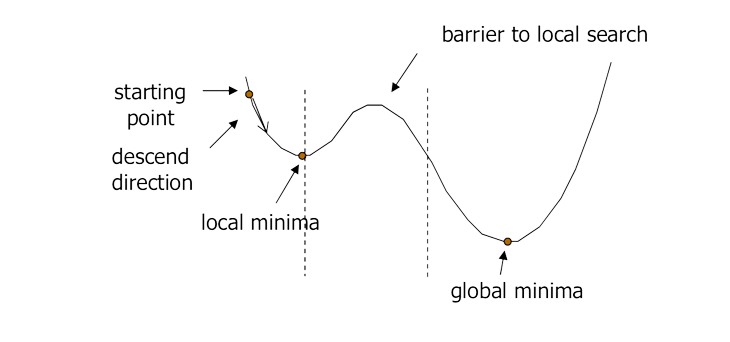
\includegraphics[width=\columnwidth]{img/simulated-annealing}

\end{frame}
\subsection{Formulazione QUBO}
\begin{frame}
  \frametitle{Problemi QUBO}

  Per essere eseguiti su macchine quantistiche, i problemi devono essere riscritti come \emph{problemi QUBO}.

  Ovvero, problemi composti da sole variabili binarie che assumono la forma:

  \begin{center}
    minimizzare 
    $\underbrace{\begin{bmatrix}
        x_1 & \cdots & x_n 
    \end{bmatrix}}_{\bar{x}^T}$ 
    $\underbrace{\begin{bmatrix}
        a_1 & \cdots & a_n \\
        \vdots & \ddots & b_n \\
        0 & \cdots & c_n 
    \end{bmatrix}}_{Q}$ 
    $\underbrace{\begin{bmatrix}
        x_1 \\
        \vdots \\
        x_n 
    \end{bmatrix}}_{\bar{x}}$       
  \end{center}

\end{frame}

\section[Da CSP a QUBO]{Min-Cut come problema QUBO}
\begin{frame}
  \frametitle{Min-Cut come problema QUBO}

  Per trasformare il problema Min-Cut in forma QUBO occorre rendere tutti i vincoli equazioni di somma zero, per cui i vincoli vengono riscritti come:

  \begin{equation*}
    \begin{array}{ll@{}ll}
    \text{minimizza}    & \displaystyle\sum_{(i, j) \in E} \omega_{ij}u_{ij}&\\
    \text{soggetto a}   & \displaystyle \pi_t - \pi_s - 1 = 0 &\\
                        & \displaystyle \pi_i - \pi_j  + \omega_{ij} - s_2 = 0\;\;\;\;\;\;\;\;\; & \forall (i,j) \in E\\
    \end{array}
\end{equation*}

\end{frame}
\begin{frame}
  \frametitle{Conversione delle variabili}

  I problemi QUBO sono caratterizzati da variabili booleane, occorre quindi convertire le variabili di slack nella loro espansione binaria.

  Nel secondo vincolo, la variabile di slack $s_2$ può assumere valori compresi tra zero e due, per questo motivo viene sostituita con $y_2^0 + 2y_2^1$, sufficiente per rappresentare i numeri nell'intervallo $[0, 3]$.

\end{frame}
\begin{frame}
  \frametitle{Rilassamento Lagrangiano}

  I vincoli del problema sono trasformati in penalità sommate alla funzione obiettivo.

  In questo modo si ottiene una singola equazione composta da variabili binarie e i rispettivi coefficienti.

\end{frame}
\begin{frame}
  \frametitle{Formulazione matematica}

  Dunque, riportiamo l'equazione del problema Min-Cut in forma QUBO:

  \begin{center}
    \begin{multline*}
      \mathcal{H}_P = \underbrace{\sum_{(u, v) \in E} \omega_{ij}u_{ij}}_{\text{Funzione obiettivo}} + \lambda(\underbrace{\pi_t - \pi_s - 1}_{\text{Primo vincolo}})^2 + \\ + \lambda\sum_{(i, j) \in E}(\underbrace{\pi_i - \pi_j + \omega_{ij} - y_2^0 - 2y_2^1}_{\text{Secondo vincolo}})^2
    \end{multline*}    
\end{center}

\end{frame}

\section{Implementazione}
\begin{frame}
  \frametitle{Struttura del codice}

  Il codice proposto è formato da uno script principale che si occupa di caricare i dati ed eseguire i diversi algoritmi testate su tutto il dataset.

  Nel pacchetto \emph{implementation} sono contenuti i metodi per l'esecuzione degli algoritmi classici e quantistici.

\end{frame}
\subsection{Test eseguiti}
\begin{frame}
  \frametitle{Sperimentazione svolta}

  L'implementazione Min-Cut in forma QUBO è stato eseguito sulla QPU della D-Wave, confrontando i tempi d'esecuzione con:
  
  \begin{enumerate}
    \item Il metodo della libreria per il calcolo del flusso massimo.
    \item Una nostra implementazione dell'algoritmo \emph{Capacity Scaling}.
  \end{enumerate} 

  Inoltre, è possibile svolgere un'indagine qualitativa per valutare pregi e difetti delle tre strategie sperimentate.

\end{frame}
\subsection{Risultati}
\begin{frame}
  \frametitle{Risultati ottenuti 1/2}

  \begin{table}
    \caption{Tempi d'esecuzione}\label{tabella_tempi}
    \centering
    \resizebox{\textwidth}{!}{
    \begin{tabular}{|r|c|c|c|}
    \hline
        Grafo & Libreria (s) & Capacity Scaling (s) & QAC (s) \\ \hline
        2015-06-10 & 0.00100 & 0.00100 & 11,37926 (0,15433) \\ \hline
        \dots & \dots & \dots & \dots \\ \hline
        2021-09-13 & 0.00001 & 0.00200 & 11,12439 (0,17091) \\ \hline\hline
        BVZ-tsukuba8$^\dagger$ & 88.28760 & 416.60800 & 81.99760 \\ \hline
        BVZ-venus1$^\dagger$ & 266.89360 & 1232.29300 & 144.78604 \\ \hline
        \dots & \dots & \dots & \dots \\ \hline
        KZ2-venus10$^\dagger$ & 1188.77692 & 14554.88358 & 759.89836 \\ \hline
        \dots & \dots & \dots & \dots \\ \hline\hline
        Media (BVZ, KZ2) & 471,75020 & 7723,76792 & 444,71604 \\ \hline
    \end{tabular}}
\end{table}

\end{frame}

\begin{frame}
  \frametitle{Risultati ottenuti 2/2}

  \begin{table}
    \caption{Flusso massimo calcolato}\label{tabella_valori}
    \centering
    \begin{tabular}{|r|c|c|}
    \hline
        Grafo & Calcolo classico & Formulazione QUBO \\ \hline
        2015-06-10 & 14 & 14 \\ \hline
        \dots & \dots & \dots \\ \hline
        2021-09-13 & 12 & 12 \\ \hline\hline
        BVZ-tsukuba8$^\dagger$ & 54458 & 111389 \\ \hline
        BVZ-venus1$^\dagger$ & 274732 & 78967 \\ \hline
        \dots & \dots & \dots \\ \hline
        KZ2-venus10$^\dagger$ & 1375201 & 2356322 \\ \hline
        \dots & \dots & \dots \\ \hline\hline
        Errore relativo & 0\% & 63,2\% \\ \hline % |val_reale - val_ottenuto|*100 / val_reale
    \end{tabular}
\end{table}

\end{frame}

\section*{Grazie per l'attenzione}

\end{document}